\section{3D Self-Supervised Methods for Medical Imaging}

\subsection*{Ссылка} \url{https://arxiv.org/abs/2006.03829}
\subsection*{Введение}
В данной работе предлагаются трехмерные варианты self-supervised 
методов, которые облегчают обучение нейронной сети на признаках 
по немаркированным трехмерным изображениям, что приводит к снижению
затрат на экспертную аннотацию. Рассмотрены 5 алгоритмов и проведен 
сравнительный анализ на трехмернвх медицинских изображениях (МРТ, КТ).
Выбор алгоритмов обусловен их успешным применением в двумерном случае и тем,
что ни один из них не был расширен до трехмерного на момент выхода статьи.

\subsection*{Основная идея}
Авторы предлагают 5 алгоритмов, которые целиком используют пространственную информацию
3D-изображения. В каждом методе используется энкодер \(g_{enc}\), который 
может быть дообучен под различные задачи.
\begin{itemize}
    \item \textbf{3D Contrastive Predictive Coding (3D-CPC)} \\
    Следуя идее, предложенной в двумерном случае, этот метод предсказывает скрытое 
    пространство для следующих (смежных) образцов. Предложенный CPC определяет 
    proxy-задачу, обрезая одинаковые по размеру и перекрывающиеся участки каждого 
    сканирования. Далее, энкодер \(g_{enc}\) сопоставляет каждый входной патч 
    \(x_{i,j,k}\) его скрытому представлению \(z_{i,j,k}= g_{enc}(x_{i,j,k})\). Затем, 
    следующая модель, называемая контекстой сетью \(g_{cxt}\) суммирует скрытые вектора патчей
    контекста \(x_{i,j,k}\) и составляет свой контекстный вектор 
    \(c_{i,j,k}=g_{cxt}(\{z_{u,v,w}\})\), где \(\{z\}\) - это множество скрытых векторов.
    Наконец, так как \(c_{i,j,k}\) захватывает высокоуровневый контент из контекста, который 
    отвечает \(x_{i,j,k}\), это позволяет предсказать скрытые представления следующих(смежных)
    патчей \(z_{i+l,j,k}\), где \(l\geq 0\). Стоит отметить, что в предложенном 3D-CPC
    в качестве \(g_{enc}\) и \(g_{cxt}\) могут использоваться сети любой архитектуры.
    \item \textbf{Relative 3D patch location (3D-RPL)} \\
    В этой задаче пространственный контекст в изображениях используется 
    как богатый источник для семантического представления данных. В предложенной 
    3D версии из каждого входного 3D изображения выбирается сетка из \(N\)
    неперекрывающихся участков \(\{x_{i}\}_{i\in \{1, \cdots N\}}\) случайного расположения. 
    Далее, центральный патч \(x_c\) используется как ссылка, а очередной патч \(x_q\)
    выбирается из окружающих \(N-1\) патчей. Далее, расположение \(x_q\) относительно \(x_c\)
    выбирается как положительная метка \(y_q\). Таким образом, задача сводится к \(N-1\)-классовой 
    классификации, где расположения оставшихся патчей используются как негативные метки.
    \item \textbf{3D Jigsaw puzzle Solving (3D-Jig)} \\
    Получение мозаичной сетки из входного изображение может рассматриваться как 
    расширение вышеприведенной задачи RPL, основанной на патчах. Пазлы формируются
    путем выбора \(nxnxn\) сетки из 3D патчей, далее эти патчи перемешиваются следуя 
    произвольной перестановк из множества предопределенных перестановок с индексом 
    \(y_{p}\in \{1,\dots , P\}\), где \(P\) - размерность множества перестановок, выбранного
    из \(n^{3}!\) всевозможных перестановок. Таким образом, задача сводится к P-классовой 
    классификации - модель тренируется просто запомнить индекс \(p\) примененной перестановки.

    \item \textbf{3D Rotation prediction (3D-Rot)} \\
    В данной задаче модель должна предсказать угол, на который повернуто изображение.
    Входное изображение поворачивается случайным образом на угол \(r\in \{1, \dots R\}\).
    Поворот изображения на угол в \(0^{o}\) вдоль трех осей произведет три идентичных версии
    исходного изображения, поэтому рассматриваются только 10 возможных поворотов из 12. 
    В таких условиях задача сводится к 10-классовой классификации.

    \item \textbf{3D Exemplar networks (3D-Exe)} \\
    Для получения supervised-меток метод опирается на аугментацию изображений. 
    Здесь для тренировочного набора данных определяется множество трансформаций 
    изображения, а новый суррогатный класс создается с помощью трансформации тренировочного 
    примера. Задача является обычной задачей классификации с кросс-энтропийной фукнцией потерь.
    Однако, с увеличением датасета и количства классов задача становится более вычислительно сложной, 
    поэтому в предложенной 3D версии внедрен механизм, который опирается на тройную
    функцию потерь.
\end{itemize}

\\
\begin{minipage}{1.0\linewidth}
    \begin{center}
        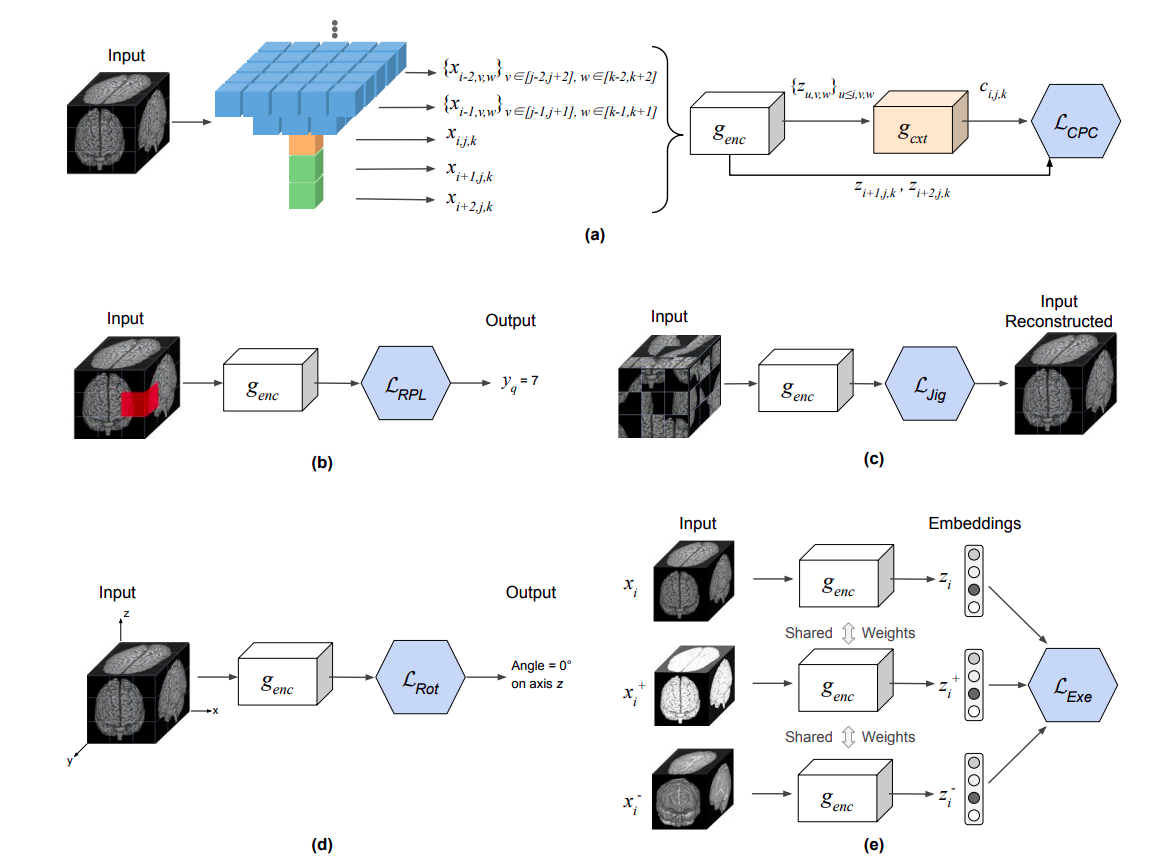
\includegraphics[scale=0.35]{ann13_arch.png} \\
        \caption{\scriptsize{(а) - 3D-CPC; (b) - 3D-RPL; (c) - 3D-Jig; (d) - 3D-Rot; (e) - 3D-Exe.}}
    \end{center}
    
\end{minipage}

\subsection*{Данные}
BraTS 2018, 3D КТ сканы с опухолями поджелудочной железы, снимки из Diabetic Retinopathy 2019 Kaggle
challenge.
\subsection*{Результаты}
 Предложенные методы были опробованы в различных медицинских задачах и показали 
 следующие результаты: \\  \\
 \textbf{1. Сегментация опухолей мозга} \\
Все предложенные методы продолевают бейзлайны, так же, как и двумерные версии этих методов.
Результаты, полученные в данной здаче показвают наличие обощающей способности
у всех предложенных методов. \\
 \begin{minipage}{1.0\linewidth}
    \begin{center}
        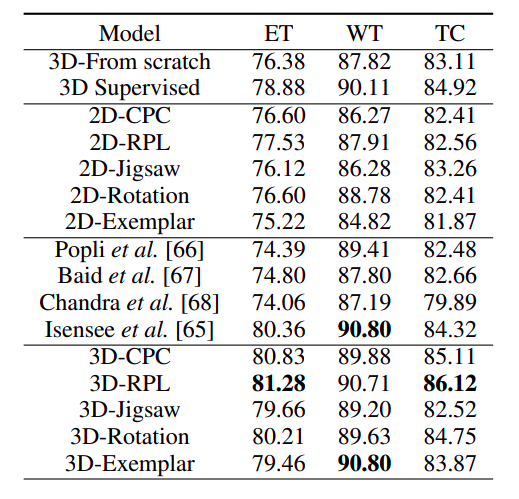
\includegraphics[scale=0.5]{ann13_res2.png} \\
        \caption{\scriptsize{Результаты сегментации BraTS}}
    \end{center}
\end{minipage} \\
\textbf{2. Сегментация опухолей поджелудочной железы} \\
Результаты, полученные с помощью предложенных методов преодолевают бейзлайны для поставленной 
задачи. Также, предложенные методы показывают достаточно быструю сходимость.

\begin{minipage}{1.0\linewidth}
    \begin{center}
        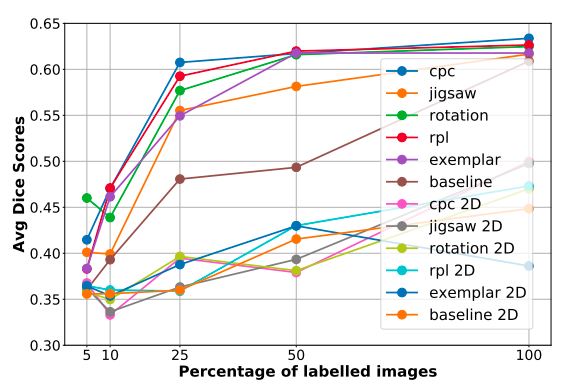
\includegraphics[scale=0.5]{ann13_panc_res.png} \\
        \caption{\scriptsize{Результаты сегментации опухолей поджелудочной железы.
        На меньшем количестве размеченных данных supervised baseline (коричневый) показывает 
        низкую обобщающую способность по сравнению с предложенными методами. Также, 3D методы 
        превосходят свои двумерные аналоги.}}
    \end{center}
\end{minipage} \\
\subsection*{Заключение}
В данной работе были продемонстрированы результаты применения предложенных 
алгоритмов в разрезе эффективности обработки данных и более быстрой сходимости.
Полученные результаты являются конкурентноспособными, а разработанные 
методы могут применяться в дальнейших исследованиях.